\subsection{Overview: High level components and their interaction}
% presentation layer, application layer, data layer
The system is divided into three main layers: presentation layer, application layer and data layer. The presentation layer is the interface between the user and the system. It is responsible for the presentation of the data and the interaction with the user. The application layer is the core of the system. It is responsible for the business logic and the comunication between the presentation layer and the data layer. The data layer is responsible for the storage of the data. It is the interface betweenm the application layer and the database.
\begin{figure}[H]
    \centering
    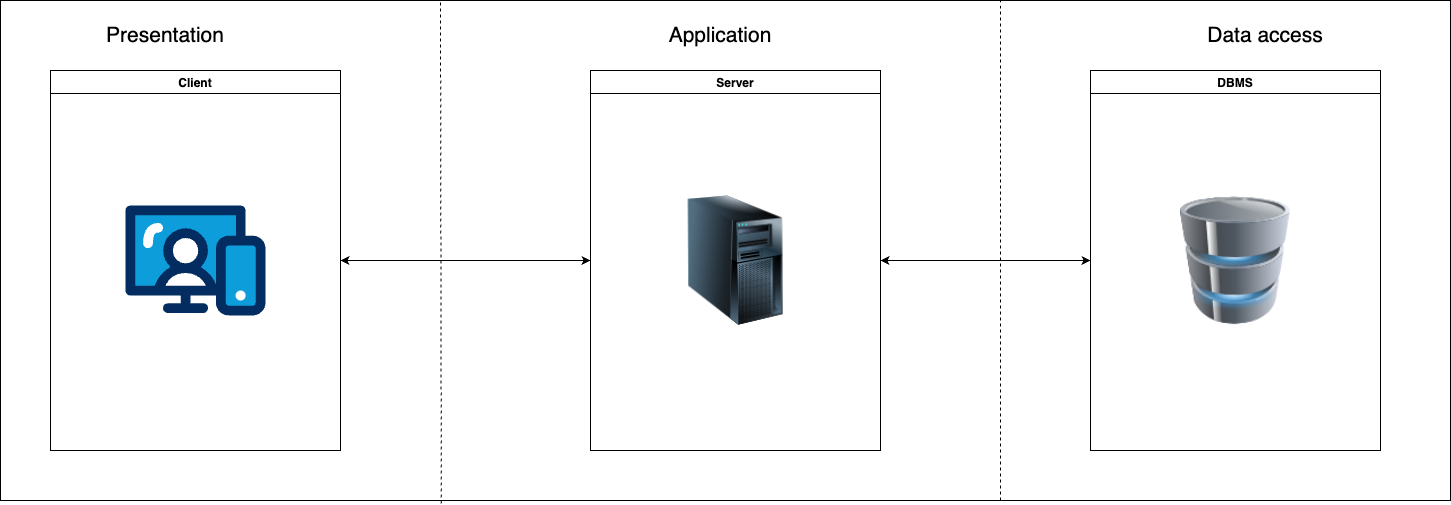
\includegraphics[width=\textwidth]{Images/three_tier.png}
    \caption{High level components and their interaction}
\end{figure}

\begin{figure}[H]
    \centering
    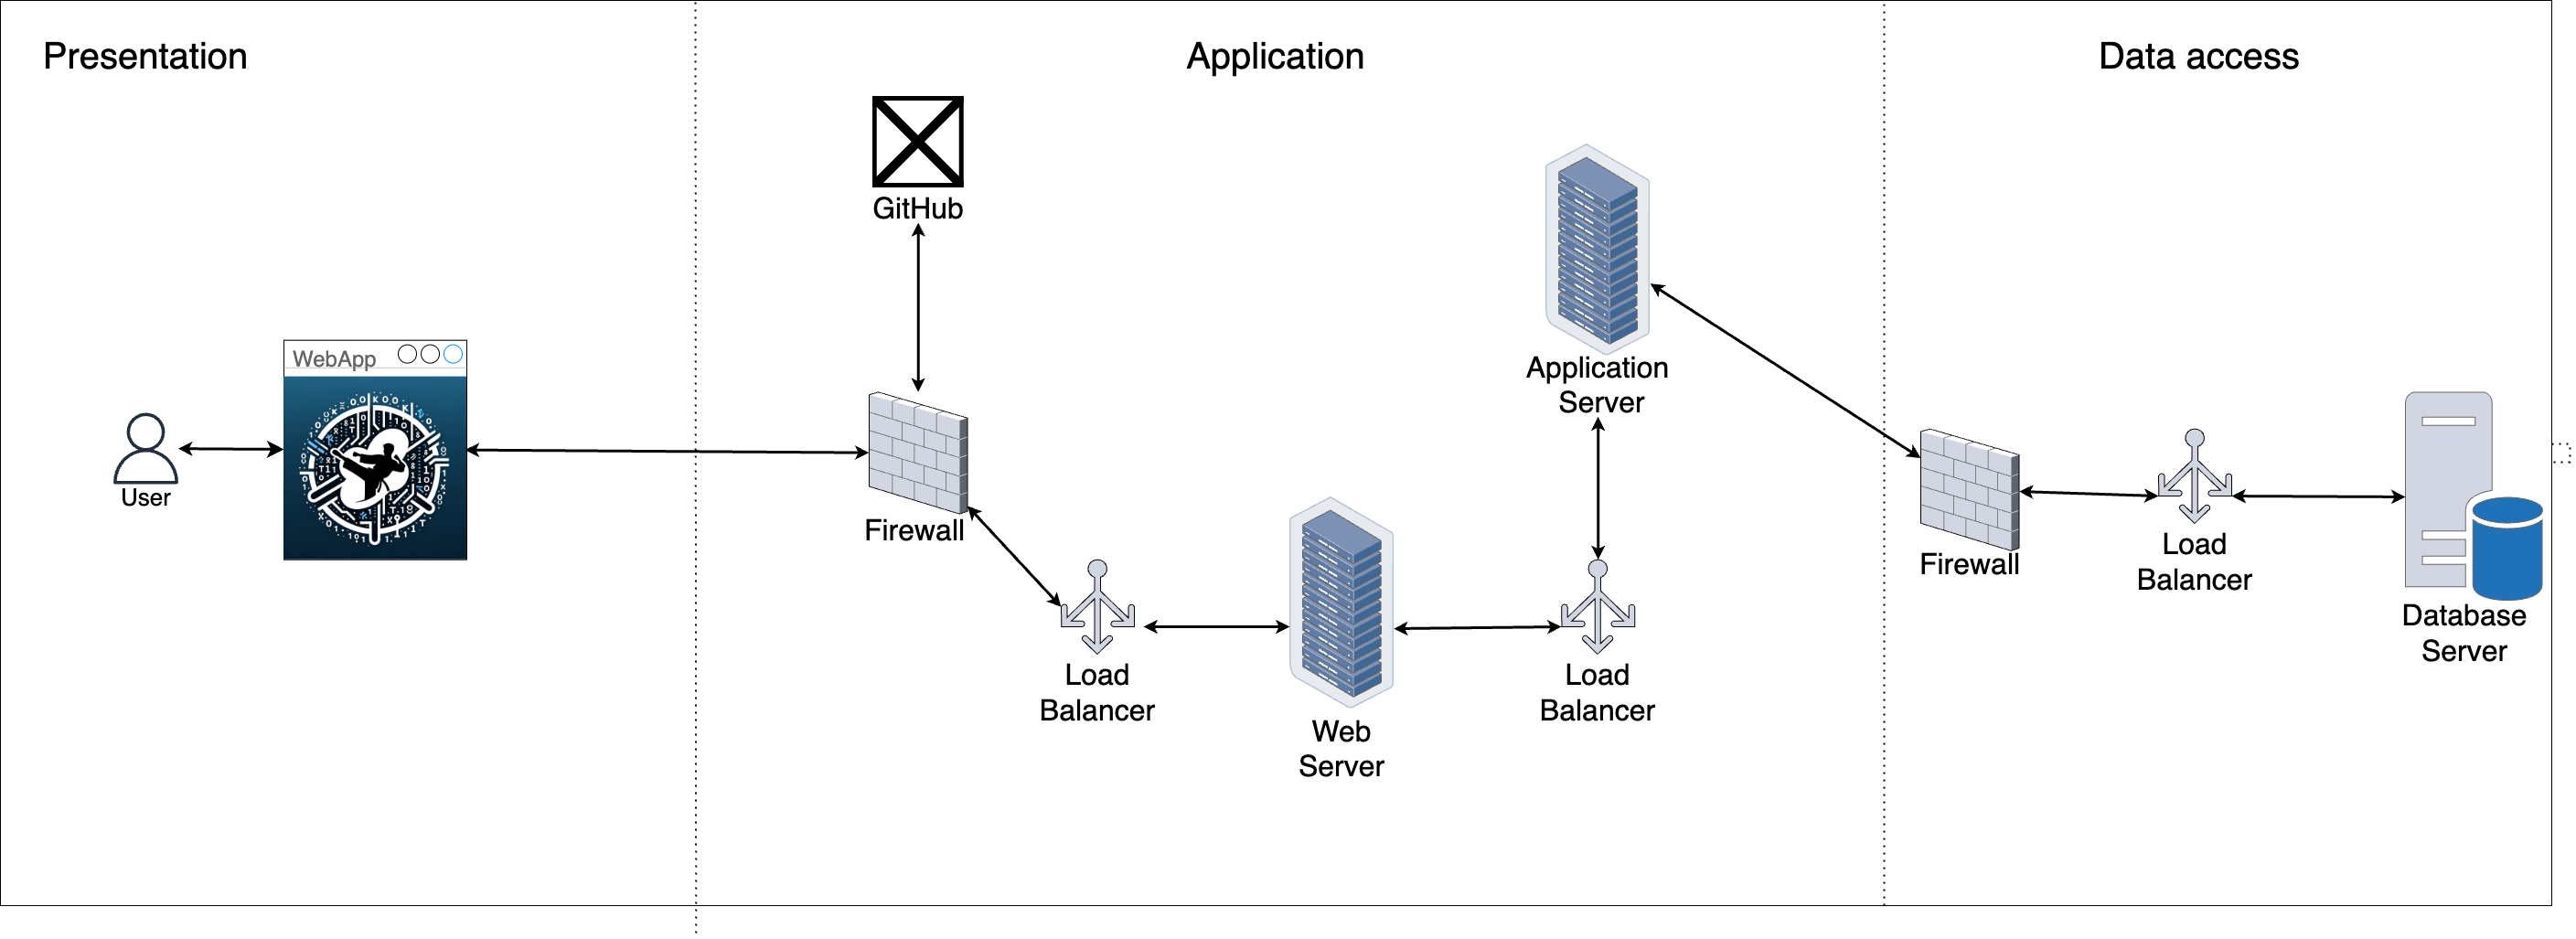
\includegraphics[width=\textwidth]{Images/high_level.png}
    \caption{Interaction between the components}
\end{figure}


\subsection{Component view}
\subsection{Deployment view}
\subsection{Component interfaces}
\subsection{Runtime view}
\subsection{Selected architectural styles and patterns}
\subsection{Other design decisions}
